% !TEX program = pdflatex
\documentclass[11pt,a4paper]{article}
\usepackage[utf8]{inputenc}
\usepackage[T1]{fontenc}
\usepackage[french]{babel}
\usepackage{lmodern,microtype,graphicx}
\usepackage[a4paper,margin=19mm,top=19mm,bottom=19mm,headheight=14pt]{geometry}
\usepackage{xcolor,tabularx,booktabs,array,enumitem,fancyhdr,titlesec,tcolorbox}
\usepackage[hidelinks]{hyperref}
\definecolor{ink}{HTML}{2B2A22}
\definecolor{gold}{HTML}{B8860B}
\definecolor{pale}{HTML}{F4EDC0}
\definecolor{muted}{HTML}{6B6B5E}
\hypersetup{pdftitle={Faire avec l'IA, garder la main sur l'image},pdfauthor={Etienne Baron},colorlinks=true,urlcolor=gold}
\pagestyle{fancy}\fancyhf{}
\fancyhead[L]{\footnotesize\textsc{Etienne Baron / SPV 2}}
\fancyhead[R]{\footnotesize Veille technologique / 11 septembre 2026}
\fancyfoot[L]{\footnotesize\color{muted}École Georges Méliès}
\fancyfoot[R]{\footnotesize\thepage\ / 4}
\renewcommand{\headrulewidth}{0.3pt}
\titleformat{\section}{\Large\bfseries\color{ink}}{\color{gold}\thesection}{0.7em}{}
\titleformat{\subsection}{\normalsize\bfseries\color{ink}}{}{0pt}{}
\titlespacing*{\section}{0pt}{0pt}{10pt}
\titlespacing*{\subsection}{0pt}{10pt}{4pt}
\setlength{\parindent}{0pt}\setlength{\parskip}{5pt}
\setlist[itemize]{leftmargin=15pt,itemsep=2pt,topsep=3pt}
\setlist[enumerate]{leftmargin=17pt,itemsep=3pt,topsep=3pt}
\newtcolorbox{focus}{colback=pale,colframe=gold,boxrule=0.5pt,arc=0pt,left=8pt,right=8pt,top=5pt,bottom=5pt}
\newcommand{\src}[1]{\textsuperscript{\textcolor{gold}{[#1]}}}
\newcolumntype{Y}{>{\raggedright\arraybackslash}X}
\begin{document}
{\small\bfseries\color{gold}VEILLE TECHNOLOGIQUE / ETIENNE BARON}\par
{\LARGE\bfseries\color{ink}Faire avec l'IA,\\garder la main sur l'image}\par
{\large Notes depuis \emph{NoClip} et \emph{NATION}}\par
\vspace{6pt}
\section{Deux films, deux façons de se perdre}
Au départ, je m'intéresse aux outils : ce qu'ils permettent de fabriquer, les passages qu'ils ouvrent entre une image tournée et une image calculée. Puis le projet résiste. Un raccord ne tient pas, le décor prend trop de place, les personnages changent. C'est là que ma veille devient utile : quand elle revient vers ce que je cherche à faire.

\textbf{\emph{NoClip}} est un court-métrage étudiant de l'École Georges Méliès. Ryan, un skateur, chute et se retrouve dans les Backrooms, un labyrinthe de couloirs jaunes. J'en ai supervisé les séquences en production virtuelle, avec un mur LED et Unreal Engine. Le problème était de faire tenir ensemble le décor numérique, la caméra et la lumière du plateau. Sans répétition technique, le défaut de tracking a été découvert au tournage. Ce cas me ramène à une question assez simple : pourquoi choisir ce dispositif si l'on n'a pas vérifié ce qu'il apporte au plan ?

\textbf{\emph{NATION}} est un projet de fiction sur lequel je mène un travail personnel de VFX, hors cadre scolaire. Pour les séquences de désert, les comédiens ont été filmés sur fond vert et la Tour est issue d'une maquette ; aucun désert n'a été tourné. Il faut donc fabriquer cet espace en post-production. Le problème se déplace : conserver les corps, faire revenir le même décor d'un plan à l'autre, intégrer le sable, le ciel et les ouvrages sans que tout se désolidarise.

\begin{center}
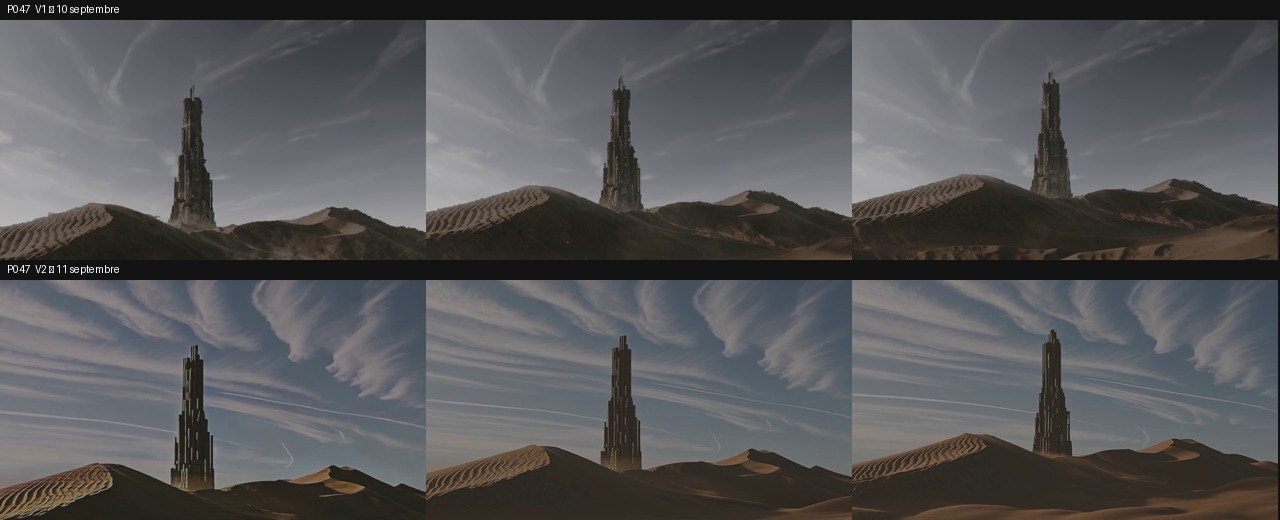
\includegraphics[width=\linewidth]{img/p047_v1_v2.jpg}
\end{center}
{\small\textbf{Plan 47 -- Trouver une référence commune.} V1 du 10 septembre en haut, V2 du 11 en bas. Le ciel change, mais la question dépasse les nuages : la Tour de ce plan devient le repère de design pour le reste de la séquence. Planches de revue NATION.}

Ces deux expériences donnent son sujet à ma veille : \textbf{comment intégrer l'IA dans une chaîne VFX sans perdre le fil du film ?} Je cherche à comprendre ce qui reste maîtrisable : les raccords, les versions, le temps passé, mais aussi les conditions d'utilisation des outils et le devenir des images qu'on leur confie.
\newpage
\section{Une veille qui revient au plan}
Je ne pars pas d'une liste de logiciels à connaître. Je pars d'une difficulté, puis je regarde autour. Comment conserver un personnage tout en changeant le fond ? Comment retrouver un résultat une semaine plus tard ? Le passage par la documentation est nécessaire, mais il ne suffit pas. Entre la fonction annoncée et le plan utilisable, il y a tout le travail d'intégration.

Les échanges avec \textbf{Creative Machines} et la jam à Creative Seeds ont nourri ce regard : les outils s'y confrontent à une intention, au temps disponible, aux choix des autres. J'y retrouve quelque chose qui m'intéresse dans la recherche : on commence avec une idée de trajet, puis ce que l'on fabrique oblige à bifurquer. Encore faut-il garder une trace de ce déplacement.

\subsection{Où je regarde, et ce que j'en garde}
Je croise les documentations d'Epic et de ComfyUI, les fiches des modèles et leurs dépôts avec les retours de fabrication et les échanges professionnels.\src{1,2} Les annonces et démonstrations servent à repérer une possibilité. Ensuite je cherche ses conditions : version, entrées nécessaires, limites, licence, matériel. Une belle sortie isolée ne dit pas combien d'essais ont été écartés.

Je garde une note courte : \emph{ce que je voulais obtenir, ce que la source promet, ce que l'essai produit}. J'y rattache le plan, son timecode, la version du traitement et une image témoin. Si la piste ne marche pas, la note reste. L'échec devient utile lorsqu'on peut comprendre ce qui a fait changer de direction.

\subsection{Donner un rythme à cette pratique}
Pour que cette veille survive aux périodes de fabrication, je la formalise ainsi :\par
{\small\renewcommand{\arraystretch}{1.15}
\begin{tabularx}{\linewidth}{@{}p{31mm}Y@{}}
\toprule
\textbf{Moment} & \textbf{Travail et trace}\\ \midrule
Chaque semaine & Une demi-heure de lecture, une demi-heure de tri ; retenir jusqu'à trois pistes reliées à un besoin réel.\\
Un essai par semaine & Une heure à une heure et demie sur un problème précis ; conserver témoin, réglages et résultat.\\
Après une retake & Dix minutes pour noter la décision, ce qui reste à reprendre et pourquoi.\\
Chaque mois & Reprendre les notes pendant trois quarts d'heure ; dégager ce qui mérite d'être partagé ou approfondi.\\
\bottomrule
\end{tabularx}}

Ce rythme est un cadre pour la suite, pas une assiduité que je reconstruis après coup. Pendant une campagne de retakes, les notes se concentrent naturellement autour des plans en cours.

\subsection{Revenir du détail à la séquence}
Je compare sur la même plage, à la même cadence, avec un témoin conservé. Le graphe ComfyUI, les modèles, les versions des nœuds et les paramètres accompagnent la sortie. Les textes et les décisions sont versionnés dans Git ; les médias restent sur les disques de production. La fiche relie les deux.

Puis je quitte l'image fixe : début, milieu, fin, lecture du plan entier et raccords voisins. C'est souvent à ce moment que la proposition se défait. Je sépare donc le contrôle technique de l'appréciation artistique : un fichier peut être complet, se lire correctement, et ne pas convenir au film. Le temps que je souhaite mesurer est celui qui mène au \textbf{plan accepté}, avec les reprises et le tri, pas seulement le temps de calcul.
\newpage
\section{Changer de méthode en regardant}
\subsection{Au plan 68, revenir aux comédiens}
\begin{center}
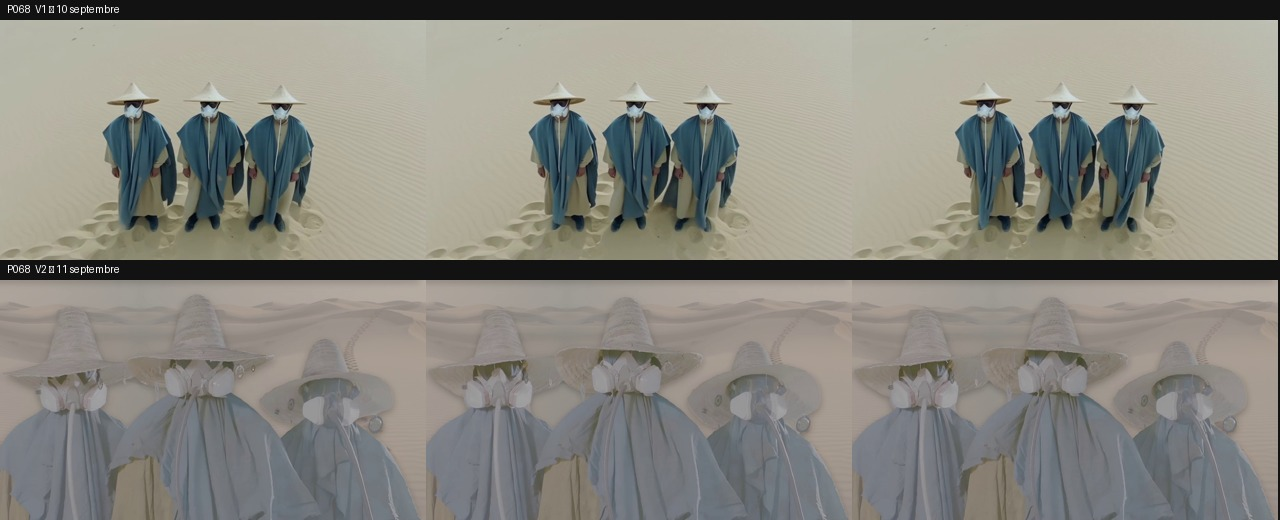
\includegraphics[width=\linewidth]{img/p068_v1_v2.jpg}
\end{center}
{\small\textbf{Plan 68 -- V1 en haut, V2 en bas.} La première proposition reconstruit les personnages. La seconde reprend les comédiens du tournage et les place sur le fond créé, avec les traces de pas. Comparatif de revue des 10 et 11 septembre.}

La V1 propose un point de vue surplombant. Mais les costumes et le cadrage demandent validation. Le brief suivant tranche : reprendre les trois personnages d'origine. Le déplacement est intéressant. On ne demande plus à la génération de porter tout le plan ; on lui laisse le décor, puis on revient au compositing pour les corps. Ce fond devient aussi celui des plans 89 et 90. Un choix local commence à organiser la séquence.

\subsection{Au plan 215, apprendre à nommer le défaut}
\noindent\begin{minipage}[t]{0.46\linewidth}
\vspace{0pt}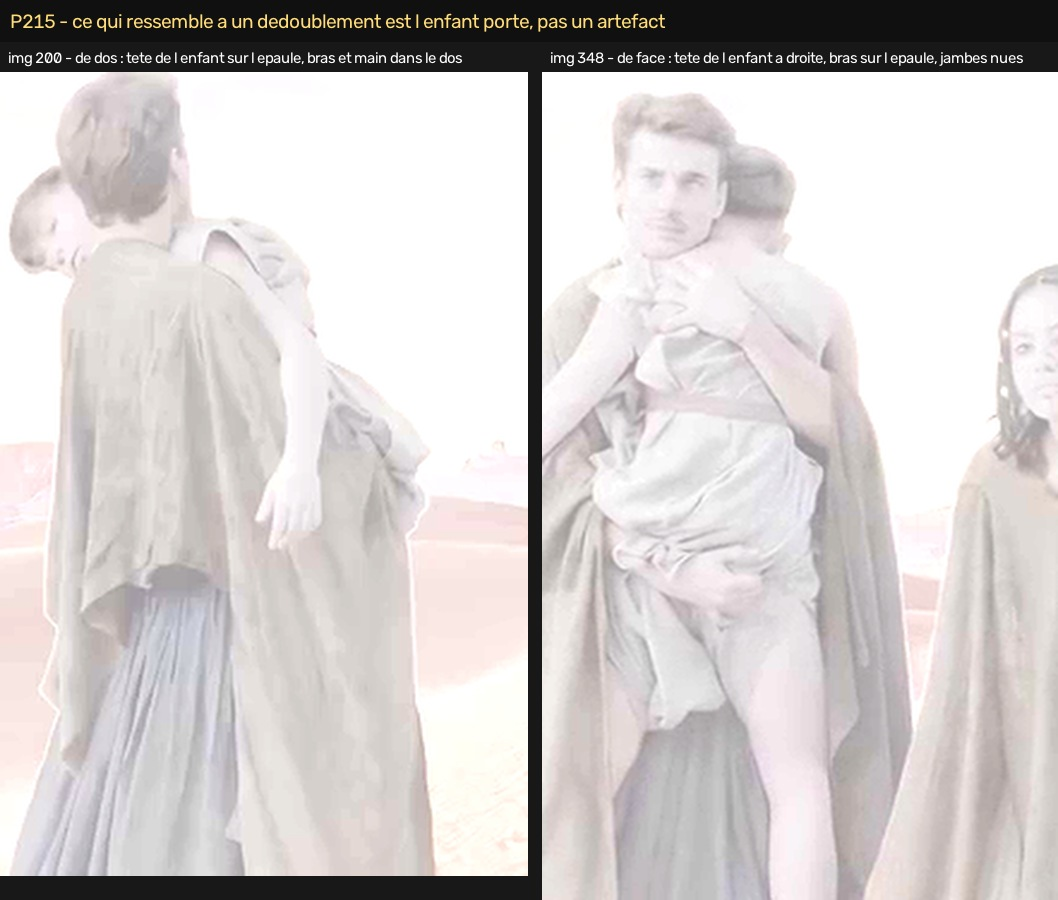
\includegraphics[width=\linewidth]{img/p215_diagnostic.jpg}
\end{minipage}\hfill
\begin{minipage}[t]{0.51\linewidth}
\vspace{0pt}\small
\textbf{Plan 215 -- L'enfant porté.} Deux instants de la planche de diagnostic du 11 septembre.

Le premier rapport parlait d'un dédoublement. En revenant aux images, le journal identifie l'enfant porté par l'homme. Effacer cette forme aurait supprimé une personne du plan.

Le problème est celui de leur séparation visuelle. La plaque personnages retrouvée conserve un contraste que le composite a perdu. Une restitution est démontrée sur les images 310 à 331, mais le suivi décroche ailleurs. Elle n'est donc pas appliquée au plan livré.

Ce détour compte dans ma veille : avant de chercher un meilleur outil, il faut parfois corriger la question.
\end{minipage}

\subsection{Garder aussi les essais écartés}
Le traitement \emph{reference-to-video}, qui associe une vidéo source et une image de référence, est retenu dans le rapport V2 pour les plans 47, 88 et 145. Sur le 215, il change l'ambiance, les costumes et fait disparaître un enfant. La production revient à un composite localisé. Le même procédé trouve ici sa place, ailleurs sa limite.

\newpage
\section{Où cette veille me conduit}
Au 11 septembre 2026, je vois surtout des outils qui se croisent. Unreal permet de travailler avec un décor lié à la caméra et un retour sur le plateau, au prix d'une préparation et d'une synchronisation exigeantes.\src{1} ComfyUI permet d'assembler des traitements ; encore faut-il raccorder leurs sorties au montage. Sur \emph{NATION}, la campagne du 10 utilise des modèles locaux, celle du 11 associe local et Comfy Cloud. Le choix ne se résume donc pas à opposer deux solutions.

Une autre piste apparaît dans le programme du \textbf{VP Gathering 2026}, tenu du 14 au 16 avril à Breda : une chaîne Chaos Arena/Vantage qui part des outils 3D pour aller vers le volume LED.\src{3,4} Elle m'intéresse parce qu'elle pose la question du passage entre les outils. Que gagne-t-on à conserver une scène dans sa chaîne de fabrication ? Je la garde comme piste à examiner, sans en déduire qu'elle conviendrait mieux à mes projets.

\subsection{Le programme comme point de rencontre}
Dans ma lecture du programme du 15 avril, trois sujets rejoignent ce travail : les décisions et les risques avant le plateau ; le passage des outils 3D au mur LED ; les compromis environnementaux de la production virtuelle.\src{3} Le premier renvoie directement à \emph{NoClip}. Le deuxième interroge la continuité des éléments. Le troisième oblige à élargir le regard : déplacer une fabrication sur des machines ne fait pas disparaître son coût matériel.

Je voudrais prolonger cette veille par un comparatif simple : une même retake traitée en compositing classique et avec une aide générative, en comptant préparation, calcul, reprises et validation. Les rapports actuels décrivent les résultats, mais ne donnent pas de mesure suffisante pour annoncer une économie globale de temps ou d'énergie.

\subsection{Une direction, pour l'instant}
Je cherche moins une chaîne capable de tout faire qu'une façon de garder prise sur ce que je fabrique. Valider un décor commun avant de le décliner. Préserver une prise de vues lorsque c'est elle qui porte la présence d'un personnage. Pouvoir retrouver une tentative et comprendre pourquoi elle a été abandonnée. Ce sont des gestes assez modestes. C'est pourtant là que cette veille rejoint, pour moi, le travail de supervision.

{\footnotesize
\textbf{Sources consultées}\par
[1] Epic Games, \href{https://dev.epicgames.com/documentation/en-us/unreal-engine/in-camera-vfx-overview-in-unreal-engine}{In-Camera VFX Overview}.\\
{}[2] ComfyUI, \href{https://docs.comfy.org/api-reference/cloud/workflow/submit-a-workflow-for-execution}{Submit a workflow for execution} (structure des graphes JSON).\\
{}[3] VP Gathering, \href{https://vpgathering.com/industry-day/}{Programme Industry Day, 15 avril 2026}.\\
{}[4] BUas / VPG, \href{https://www.b2match.com/e/vp-gathering-2026/components/65001}{Présentation de l'édition 2026}. Pages web consultées le 11/09/2026.\\
\textbf{Matériau de terrain :} NATION, rapports de conformation et de livraison du 10 septembre ; brief V2, état de livraison et journal du 11 septembre 2026. Les trois figures proviennent des planches de contrôle V2 ; il s'agit de versions de revue.
}

\vspace{5pt}
\begin{focus}
\footnotesize\textbf{Transparence -- assistance par intelligence artificielle.}
En référence à l'article 50 du \href{https://eur-lex.europa.eu/eli/reg/2024/1689/oj?locale=fr}{règlement européen sur l'IA (AI Act, UE 2024/1689)}, je signale l'usage d'IA générative et agentique pour aider à la rédaction, à la structuration et à la mise en forme LaTeX de ce document. Les images de NATION présentées associent prises de vues réelles, éléments générés ou transformés par IA et compositing. Les choix artistiques, la validation du texte et la responsabilité éditoriale restent les miens.
\end{focus}
\end{document}
